\documentclass[twoside]{book}

% Packages required by doxygen
\usepackage{fixltx2e}
\usepackage{calc}
\usepackage{doxygen}
\usepackage[export]{adjustbox} % also loads graphicx
\usepackage{graphicx}
\usepackage[utf8]{inputenc}
\usepackage{makeidx}
\usepackage{multicol}
\usepackage{multirow}
\PassOptionsToPackage{warn}{textcomp}
\usepackage{textcomp}
\usepackage[nointegrals]{wasysym}
\usepackage[table]{xcolor}

% Font selection
\usepackage[T1]{fontenc}
\usepackage[scaled=.90]{helvet}
\usepackage{courier}
\usepackage{amssymb}
\usepackage{sectsty}
\renewcommand{\familydefault}{\sfdefault}
\allsectionsfont{%
  \fontseries{bc}\selectfont%
  \color{darkgray}%
}
\renewcommand{\DoxyLabelFont}{%
  \fontseries{bc}\selectfont%
  \color{darkgray}%
}
\newcommand{\+}{\discretionary{\mbox{\scriptsize$\hookleftarrow$}}{}{}}

% Page & text layout
\usepackage{geometry}
\geometry{%
  a4paper,%
  top=2.5cm,%
  bottom=2.5cm,%
  left=2.5cm,%
  right=2.5cm%
}
\tolerance=750
\hfuzz=15pt
\hbadness=750
\setlength{\emergencystretch}{15pt}
\setlength{\parindent}{0cm}
\setlength{\parskip}{3ex plus 2ex minus 2ex}
\makeatletter
\renewcommand{\paragraph}{%
  \@startsection{paragraph}{4}{0ex}{-1.0ex}{1.0ex}{%
    \normalfont\normalsize\bfseries\SS@parafont%
  }%
}
\renewcommand{\subparagraph}{%
  \@startsection{subparagraph}{5}{0ex}{-1.0ex}{1.0ex}{%
    \normalfont\normalsize\bfseries\SS@subparafont%
  }%
}
\makeatother

% Headers & footers
\usepackage{fancyhdr}
\pagestyle{fancyplain}
\fancyhead[LE]{\fancyplain{}{\bfseries\thepage}}
\fancyhead[CE]{\fancyplain{}{}}
\fancyhead[RE]{\fancyplain{}{\bfseries\leftmark}}
\fancyhead[LO]{\fancyplain{}{\bfseries\rightmark}}
\fancyhead[CO]{\fancyplain{}{}}
\fancyhead[RO]{\fancyplain{}{\bfseries\thepage}}
\fancyfoot[LE]{\fancyplain{}{}}
\fancyfoot[CE]{\fancyplain{}{}}
\fancyfoot[RE]{\fancyplain{}{\bfseries\scriptsize Generated by Doxygen }}
\fancyfoot[LO]{\fancyplain{}{\bfseries\scriptsize Generated by Doxygen }}
\fancyfoot[CO]{\fancyplain{}{}}
\fancyfoot[RO]{\fancyplain{}{}}
\renewcommand{\footrulewidth}{0.4pt}
\renewcommand{\chaptermark}[1]{%
  \markboth{#1}{}%
}
\renewcommand{\sectionmark}[1]{%
  \markright{\thesection\ #1}%
}

% Indices & bibliography
\usepackage{natbib}
\usepackage[titles]{tocloft}
\setcounter{tocdepth}{3}
\setcounter{secnumdepth}{5}
\makeindex

% Hyperlinks (required, but should be loaded last)
\usepackage{ifpdf}
\ifpdf
  \usepackage[pdftex,pagebackref=true]{hyperref}
\else
  \usepackage[ps2pdf,pagebackref=true]{hyperref}
\fi
\hypersetup{%
  colorlinks=true,%
  linkcolor=blue,%
  citecolor=blue,%
  unicode%
}

% Custom commands
\newcommand{\clearemptydoublepage}{%
  \newpage{\pagestyle{empty}\cleardoublepage}%
}

\usepackage{caption}
\captionsetup{labelsep=space,justification=centering,font={bf},singlelinecheck=off,skip=4pt,position=top}

%===== C O N T E N T S =====

\begin{document}

% Titlepage & ToC
\hypersetup{pageanchor=false,
             bookmarksnumbered=true,
             pdfencoding=unicode
            }
\pagenumbering{roman}
\begin{titlepage}
\vspace*{7cm}
\begin{center}%
{\Large First node }\\
\vspace*{1cm}
{\large Generated by Doxygen 1.8.11}\\
\end{center}
\end{titlepage}
\clearemptydoublepage
\tableofcontents
\clearemptydoublepage
\pagenumbering{arabic}
\hypersetup{pageanchor=true}

%--- Begin generated contents ---
\chapter{Research Track I -\/ first assignment}
\label{md_src_assignment1_README}
\hypertarget{md_src_assignment1_README}{}
The assignment requires controlling a holonomic robot in a 2d space with a simple 2d simulator, Stage. The simulator can be launched by executing the command\+:


\begin{DoxyCode}
1 rosrun stage\_ros stageros $(rospack find assignment1)/world/exercise.world
\end{DoxyCode}


\subsubsection*{The following behaviour should be achieved}


\begin{DoxyItemize}
\item 1. The robot asks for a random target, with both coordinates in the interval (-\/6.\+0, 6.\+0).
\item 2. The robot reaches the target.
\item 3. Go to step 1.
\end{DoxyItemize}

\subsubsection*{Consider the following requirements}


\begin{DoxyItemize}
\item A new R\+OS packages should be created.
\item Two processes (R\+OS nodes) should be developed.
\item You may use cpp or python for writing your code.
\item The first process will be in charge of\+:
\begin{DoxyItemize}
\item calling a service for receiving a random target;
\item making the robot reach the target.
\end{DoxyItemize}
\item The second process will act as a Service Server, by replying to the client with a random target, having x and y in the interval (-\/6.\+0, 6.\+0).
\item A target is considered reached when the distance between the robot and the target is below 0.\+1.
\end{DoxyItemize}

\subsubsection*{Some hints}


\begin{DoxyItemize}
\item The first node should implement a R\+OS publisher (cmd\+\_\+vel, for setting the robot speed), a R\+OS subscriber (odom, for knowing the actual robot position) and a R\+OS client (for receiving the random target)
\item The second node should implement a R\+OS server (for setting the random target)
\item The position of the robot is given in the topic {\bfseries odom}, by using a {\bfseries nav\+\_\+msgs/\+Odometry} (Odometry message defined in the package nav\+\_\+msgs) message. This means that the x and y position of the robot may be retrieved by reading the pose.\+pose.\+position.\+x and pose.\+pose.\+position.\+y fields of the message received by the callback associated with the subscriber.
\item For the robot control, at first, check if the position has been reached. If yes, you should call the service to retrieve the new target position. If not, you should set {\bfseries cmd\+\_\+vel} (a {\bfseries geometry\+\_\+msgs/\+Twist} message) depending on the difference between the target (xt) and the robot position (x) (e.\+g., vel\+\_\+x = k$\ast$ (xt -\/ x))
\end{DoxyItemize}

\subsubsection*{How to submit the assignment\+:}


\begin{DoxyItemize}
\item The link of a github repository containing the developed R\+OS package should be given;
\item The repo should have a \hyperlink{_r_e_a_d_m_e_8md}{R\+E\+A\+D\+M\+E.\+md} file with\+:
\begin{DoxyItemize}
\item Description of the content of the package (nodes, custom messages or services (if any)).
\item Computational graph of the system (how do nodes communicate? You may use rqt\+\_\+graph).
\item Instructions about how to run the code.
\end{DoxyItemize}
\item Functions and source files should be documented (optional\+: you can create a docs folder with Doxy\+Gen documentation).
\end{DoxyItemize}

\subsubsection*{Deadline}

A soft deadline is set to the 25th November and the next Research Track class will be on November 26th. This means that\+:
\begin{DoxyItemize}
\item You can actually submit your assignment at any time, however 10 days before the oral discussion.
\item I strongly advise you to start working on the assignment in the next weeks. Indeed, in the last 9 hours of the course, we are going to work on more complex robotic simulations, which require a good knowledge of R\+OS. Doing the assignment will be a good way to understand what it is still unclear and catch up with the course.
\item In the next two weeks, you can contact me even outside class hours for clarifications about the assignment and the course subjects in general. 
\end{DoxyItemize}
\chapter{File Index}
\section{File List}
Here is a list of all files with brief descriptions\+:\begin{DoxyCompactList}
\item\contentsline{section}{src/assignment/src/\hyperlink{first_8cpp}{first.\+cpp} }{\pageref{first_8cpp}}{}
\item\contentsline{section}{src/my\+\_\+srv/src/\hyperlink{harmonic__server_8cpp}{harmonic\+\_\+server.\+cpp} }{\pageref{harmonic__server_8cpp}}{}
\item\contentsline{section}{src/my\+\_\+srv/src/\hyperlink{randpos__server_8cpp}{randpos\+\_\+server.\+cpp} }{\pageref{randpos__server_8cpp}}{}
\item\contentsline{section}{src/my\+\_\+srv/src/\hyperlink{velocity__server_8cpp}{velocity\+\_\+server.\+cpp} }{\pageref{velocity__server_8cpp}}{}
\end{DoxyCompactList}

\chapter{File Documentation}
\hypertarget{first_8cpp}{}\section{src/assignment/src/first.cpp File Reference}
\label{first_8cpp}\index{src/assignment/src/first.\+cpp@{src/assignment/src/first.\+cpp}}
{\ttfamily \#include \char`\"{}ros/ros.\+h\char`\"{}}\\*
{\ttfamily \#include \char`\"{}geometry\+\_\+msgs/\+Twist.\+h\char`\"{}}\\*
{\ttfamily \#include \char`\"{}nav\+\_\+msgs/\+Odometry.\+h\char`\"{}}\\*
{\ttfamily \#include \char`\"{}my\+\_\+srv/\+Randpos.\+h\char`\"{}}\\*
Include dependency graph for first.\+cpp\+:
\nopagebreak
\begin{figure}[H]
\begin{center}
\leavevmode
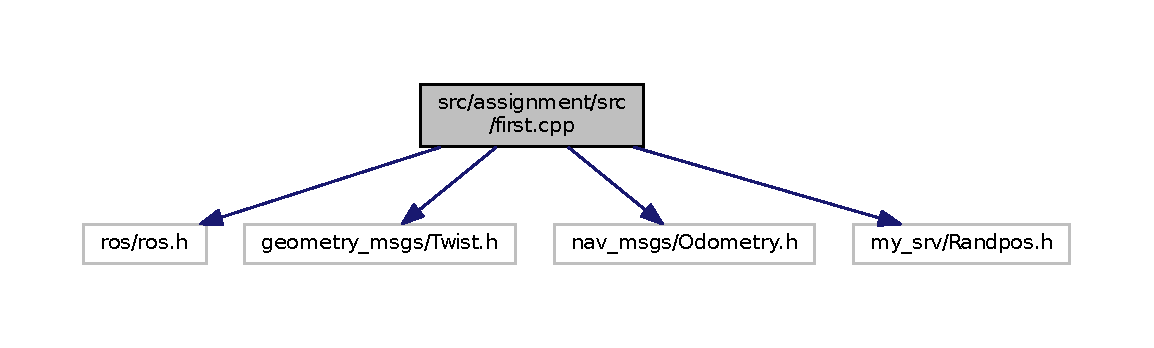
\includegraphics[width=350pt]{first_8cpp__incl}
\end{center}
\end{figure}
\subsection*{Functions}
\begin{DoxyCompactItemize}
\item 
void \hyperlink{first_8cpp_aab6e381bffc34921244a29ec0538ba64}{position\+Callback} (const nav\+\_\+msgs\+::\+Odometry\+::\+Const\+Ptr \&msg)
\item 
int \hyperlink{first_8cpp_a3c04138a5bfe5d72780bb7e82a18e627}{main} (int argc, char $\ast$$\ast$argv)
\end{DoxyCompactItemize}
\subsection*{Variables}
\begin{DoxyCompactItemize}
\item 
ros\+::\+Publisher \hyperlink{first_8cpp_ac050ecd28d14458e8d356e5f6d38a25b}{chatter\+\_\+pub}
\item 
ros\+::\+Service\+Client \hyperlink{first_8cpp_a17bcd065930a8a7f9f194078d9977268}{client}
\item 
my\+\_\+srv\+::\+Randpos \hyperlink{first_8cpp_a71b52081906c5c95f08fe23019c5dd56}{rec\+\_\+randpos}
\item 
float \hyperlink{first_8cpp_a4b312b3530217eb51cbad6e930610f6b}{vel\+\_\+x}
\item 
float \hyperlink{first_8cpp_a1dd0876197a1e2dba35d41d6a6d9eab4}{vel\+\_\+y}
\item 
float \hyperlink{first_8cpp_a9d466da6de3ce8a6002eeb6ac47204a6}{randpos\+\_\+x}
\item 
float \hyperlink{first_8cpp_aad13f1b6016597150e885f101c9ff9f6}{randpos\+\_\+y}
\item 
geometry\+\_\+msgs\+::\+Twist \hyperlink{first_8cpp_af111fcabf9f8b38b69faa049d84be60d}{msg\+\_\+sent}
\end{DoxyCompactItemize}


\subsection{Function Documentation}
\index{first.\+cpp@{first.\+cpp}!main@{main}}
\index{main@{main}!first.\+cpp@{first.\+cpp}}
\subsubsection[{\texorpdfstring{main(int argc, char $\ast$$\ast$argv)}{main(int argc, char **argv)}}]{\setlength{\rightskip}{0pt plus 5cm}int main (
\begin{DoxyParamCaption}
\item[{int}]{argc, }
\item[{char $\ast$$\ast$}]{argv}
\end{DoxyParamCaption}
)}\hypertarget{first_8cpp_a3c04138a5bfe5d72780bb7e82a18e627}{}\label{first_8cpp_a3c04138a5bfe5d72780bb7e82a18e627}
The ros\+::init() function needs to see argc and argv so that it can perform any R\+OS arguments and name remapping that were provided at the command line.

Node\+Handle is the main access point to communications with the R\+OS system.

Here the client is created over getting a random position over the /randpos service

Here it is signaled that the program will publish the velocity on the topic /cmd\+\_\+vel

In order to get a first random position and start moving the robot, before the subscribe is made, the random position is requested once. It is the same logic as explained in the end of the callback function

Here you are declaring the subscription to the topic /odom and calling the callback

ros\+::spin() will enter a loop, pumping callbacks. \index{first.\+cpp@{first.\+cpp}!position\+Callback@{position\+Callback}}
\index{position\+Callback@{position\+Callback}!first.\+cpp@{first.\+cpp}}
\subsubsection[{\texorpdfstring{position\+Callback(const nav\+\_\+msgs\+::\+Odometry\+::\+Const\+Ptr \&msg)}{positionCallback(const nav_msgs::Odometry::ConstPtr &msg)}}]{\setlength{\rightskip}{0pt plus 5cm}void position\+Callback (
\begin{DoxyParamCaption}
\item[{const nav\+\_\+msgs\+::\+Odometry\+::\+Const\+Ptr \&}]{msg}
\end{DoxyParamCaption}
)}\hypertarget{first_8cpp_aab6e381bffc34921244a29ec0538ba64}{}\label{first_8cpp_aab6e381bffc34921244a29ec0538ba64}
Message type twist for the velocity In this callback the actual position of the robot is updated with every loop. This position is compared with the target position and if the target hasn´t been reached beyond the stablished boundaries, the velocity is set. Else, the robot is stopped by setting a velocity of 0 and a new target position is requested. With this, the loop is reestarted

Here the distance/ velocity of the robot is computed for every loop and then printed in the screen. As the specification of the constant k was let to the programmer, in order to do the coding easier it has been defined as 1, like that, both distance and velocity remain equal

In this section of the code, there are 2 kind of \char`\"{}ifs\char`\"{}, the ones concerning the X coordinate and the ones regarding the Y coordinate. With this code, it is verified if the distance between the robot and the target coordinates are outside the boundaries or not, and depending on it the velocity is set with the given formula or is set to 0 respectively. Then the velocity is published for the robot to start moving

In this section of the code, it is verified if the target has been reached, and if so, a new random position is requested (called) sending the maximum and minimum boundaries for the random number, and receiving said number in the variables randpos\+\_\+x and randpos\+\_\+y 

\subsection{Variable Documentation}
\index{first.\+cpp@{first.\+cpp}!chatter\+\_\+pub@{chatter\+\_\+pub}}
\index{chatter\+\_\+pub@{chatter\+\_\+pub}!first.\+cpp@{first.\+cpp}}
\subsubsection[{\texorpdfstring{chatter\+\_\+pub}{chatter_pub}}]{\setlength{\rightskip}{0pt plus 5cm}ros\+::\+Publisher chatter\+\_\+pub}\hypertarget{first_8cpp_ac050ecd28d14458e8d356e5f6d38a25b}{}\label{first_8cpp_ac050ecd28d14458e8d356e5f6d38a25b}
This program receives a random position and controlls the velocity of the robot to reach said target \index{first.\+cpp@{first.\+cpp}!client@{client}}
\index{client@{client}!first.\+cpp@{first.\+cpp}}
\subsubsection[{\texorpdfstring{client}{client}}]{\setlength{\rightskip}{0pt plus 5cm}ros\+::\+Service\+Client client}\hypertarget{first_8cpp_a17bcd065930a8a7f9f194078d9977268}{}\label{first_8cpp_a17bcd065930a8a7f9f194078d9977268}
Publisher for the velocity of the robot \index{first.\+cpp@{first.\+cpp}!msg\+\_\+sent@{msg\+\_\+sent}}
\index{msg\+\_\+sent@{msg\+\_\+sent}!first.\+cpp@{first.\+cpp}}
\subsubsection[{\texorpdfstring{msg\+\_\+sent}{msg_sent}}]{\setlength{\rightskip}{0pt plus 5cm}geometry\+\_\+msgs\+::\+Twist msg\+\_\+sent}\hypertarget{first_8cpp_af111fcabf9f8b38b69faa049d84be60d}{}\label{first_8cpp_af111fcabf9f8b38b69faa049d84be60d}
due to the election of K=1 as velocity constant, vel\+\_\+x and vel\+\_\+y are both the velocity of the robot and the distance with the target; while randpos\+\_\+x and \+\_\+randpos\+\_\+y are the target random positions \index{first.\+cpp@{first.\+cpp}!randpos\+\_\+x@{randpos\+\_\+x}}
\index{randpos\+\_\+x@{randpos\+\_\+x}!first.\+cpp@{first.\+cpp}}
\subsubsection[{\texorpdfstring{randpos\+\_\+x}{randpos_x}}]{\setlength{\rightskip}{0pt plus 5cm}float randpos\+\_\+x}\hypertarget{first_8cpp_a9d466da6de3ce8a6002eeb6ac47204a6}{}\label{first_8cpp_a9d466da6de3ce8a6002eeb6ac47204a6}
\index{first.\+cpp@{first.\+cpp}!randpos\+\_\+y@{randpos\+\_\+y}}
\index{randpos\+\_\+y@{randpos\+\_\+y}!first.\+cpp@{first.\+cpp}}
\subsubsection[{\texorpdfstring{randpos\+\_\+y}{randpos_y}}]{\setlength{\rightskip}{0pt plus 5cm}float randpos\+\_\+y}\hypertarget{first_8cpp_aad13f1b6016597150e885f101c9ff9f6}{}\label{first_8cpp_aad13f1b6016597150e885f101c9ff9f6}
\index{first.\+cpp@{first.\+cpp}!rec\+\_\+randpos@{rec\+\_\+randpos}}
\index{rec\+\_\+randpos@{rec\+\_\+randpos}!first.\+cpp@{first.\+cpp}}
\subsubsection[{\texorpdfstring{rec\+\_\+randpos}{rec_randpos}}]{\setlength{\rightskip}{0pt plus 5cm}my\+\_\+srv\+::\+Randpos rec\+\_\+randpos}\hypertarget{first_8cpp_a71b52081906c5c95f08fe23019c5dd56}{}\label{first_8cpp_a71b52081906c5c95f08fe23019c5dd56}
Client for receiving the random targer \index{first.\+cpp@{first.\+cpp}!vel\+\_\+x@{vel\+\_\+x}}
\index{vel\+\_\+x@{vel\+\_\+x}!first.\+cpp@{first.\+cpp}}
\subsubsection[{\texorpdfstring{vel\+\_\+x}{vel_x}}]{\setlength{\rightskip}{0pt plus 5cm}float vel\+\_\+x}\hypertarget{first_8cpp_a4b312b3530217eb51cbad6e930610f6b}{}\label{first_8cpp_a4b312b3530217eb51cbad6e930610f6b}
Message type received from the server \index{first.\+cpp@{first.\+cpp}!vel\+\_\+y@{vel\+\_\+y}}
\index{vel\+\_\+y@{vel\+\_\+y}!first.\+cpp@{first.\+cpp}}
\subsubsection[{\texorpdfstring{vel\+\_\+y}{vel_y}}]{\setlength{\rightskip}{0pt plus 5cm}float vel\+\_\+y}\hypertarget{first_8cpp_a1dd0876197a1e2dba35d41d6a6d9eab4}{}\label{first_8cpp_a1dd0876197a1e2dba35d41d6a6d9eab4}

\hypertarget{_r_e_a_d_m_e_8md}{}\section{src/assignment1/\+R\+E\+A\+D\+ME.md File Reference}
\label{_r_e_a_d_m_e_8md}\index{src/assignment1/\+R\+E\+A\+D\+M\+E.\+md@{src/assignment1/\+R\+E\+A\+D\+M\+E.\+md}}

\hypertarget{harmonic__server_8cpp}{}\section{src/my\+\_\+srv/src/harmonic\+\_\+server.cpp File Reference}
\label{harmonic__server_8cpp}\index{src/my\+\_\+srv/src/harmonic\+\_\+server.\+cpp@{src/my\+\_\+srv/src/harmonic\+\_\+server.\+cpp}}
{\ttfamily \#include \char`\"{}ros/ros.\+h\char`\"{}}\\*
{\ttfamily \#include \char`\"{}my\+\_\+srv/\+Harmonic.\+h\char`\"{}}\\*
{\ttfamily \#include $<$math.\+h$>$}\\*
Include dependency graph for harmonic\+\_\+server.\+cpp\+:
\nopagebreak
\begin{figure}[H]
\begin{center}
\leavevmode
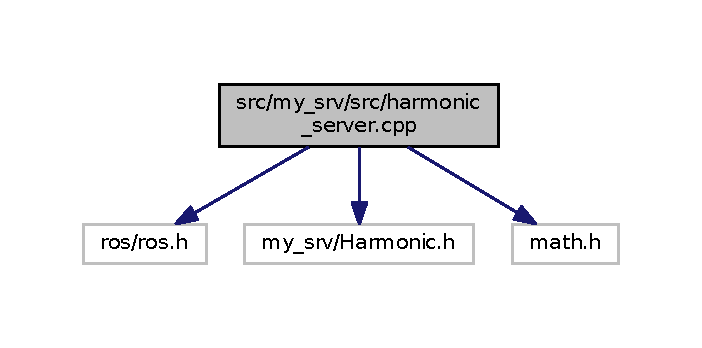
\includegraphics[width=337pt]{harmonic__server_8cpp__incl}
\end{center}
\end{figure}
\subsection*{Macros}
\begin{DoxyCompactItemize}
\item 
\#define \hyperlink{harmonic__server_8cpp_a598a3330b3c21701223ee0ca14316eca}{PI}~3.\+14159265358979323846
\end{DoxyCompactItemize}
\subsection*{Functions}
\begin{DoxyCompactItemize}
\item 
bool \hyperlink{harmonic__server_8cpp_a6526041a2d4c39b50db703597fdd40f8}{harmonic} (my\+\_\+srv\+::\+Harmonic\+::\+Request \&req, my\+\_\+srv\+::\+Harmonic\+::\+Response \&res)
\item 
int \hyperlink{harmonic__server_8cpp_a3c04138a5bfe5d72780bb7e82a18e627}{main} (int argc, char $\ast$$\ast$argv)
\end{DoxyCompactItemize}


\subsection{Macro Definition Documentation}
\index{harmonic\+\_\+server.\+cpp@{harmonic\+\_\+server.\+cpp}!PI@{PI}}
\index{PI@{PI}!harmonic\+\_\+server.\+cpp@{harmonic\+\_\+server.\+cpp}}
\subsubsection[{\texorpdfstring{PI}{PI}}]{\setlength{\rightskip}{0pt plus 5cm}\#define PI~3.\+14159265358979323846}\hypertarget{harmonic__server_8cpp_a598a3330b3c21701223ee0ca14316eca}{}\label{harmonic__server_8cpp_a598a3330b3c21701223ee0ca14316eca}


\subsection{Function Documentation}
\index{harmonic\+\_\+server.\+cpp@{harmonic\+\_\+server.\+cpp}!harmonic@{harmonic}}
\index{harmonic@{harmonic}!harmonic\+\_\+server.\+cpp@{harmonic\+\_\+server.\+cpp}}
\subsubsection[{\texorpdfstring{harmonic(my\+\_\+srv\+::\+Harmonic\+::\+Request \&req, my\+\_\+srv\+::\+Harmonic\+::\+Response \&res)}{harmonic(my_srv::Harmonic::Request &req, my_srv::Harmonic::Response &res)}}]{\setlength{\rightskip}{0pt plus 5cm}bool harmonic (
\begin{DoxyParamCaption}
\item[{my\+\_\+srv\+::\+Harmonic\+::\+Request \&}]{req, }
\item[{my\+\_\+srv\+::\+Harmonic\+::\+Response \&}]{res}
\end{DoxyParamCaption}
)}\hypertarget{harmonic__server_8cpp_a6526041a2d4c39b50db703597fdd40f8}{}\label{harmonic__server_8cpp_a6526041a2d4c39b50db703597fdd40f8}
\index{harmonic\+\_\+server.\+cpp@{harmonic\+\_\+server.\+cpp}!main@{main}}
\index{main@{main}!harmonic\+\_\+server.\+cpp@{harmonic\+\_\+server.\+cpp}}
\subsubsection[{\texorpdfstring{main(int argc, char $\ast$$\ast$argv)}{main(int argc, char **argv)}}]{\setlength{\rightskip}{0pt plus 5cm}int main (
\begin{DoxyParamCaption}
\item[{int}]{argc, }
\item[{char $\ast$$\ast$}]{argv}
\end{DoxyParamCaption}
)}\hypertarget{harmonic__server_8cpp_a3c04138a5bfe5d72780bb7e82a18e627}{}\label{harmonic__server_8cpp_a3c04138a5bfe5d72780bb7e82a18e627}

\hypertarget{randpos__server_8cpp}{}\section{src/my\+\_\+srv/src/randpos\+\_\+server.cpp File Reference}
\label{randpos__server_8cpp}\index{src/my\+\_\+srv/src/randpos\+\_\+server.\+cpp@{src/my\+\_\+srv/src/randpos\+\_\+server.\+cpp}}
{\ttfamily \#include \char`\"{}ros/ros.\+h\char`\"{}}\\*
{\ttfamily \#include \char`\"{}my\+\_\+srv/\+Randpos.\+h\char`\"{}}\\*
Include dependency graph for randpos\+\_\+server.\+cpp\+:
\nopagebreak
\begin{figure}[H]
\begin{center}
\leavevmode
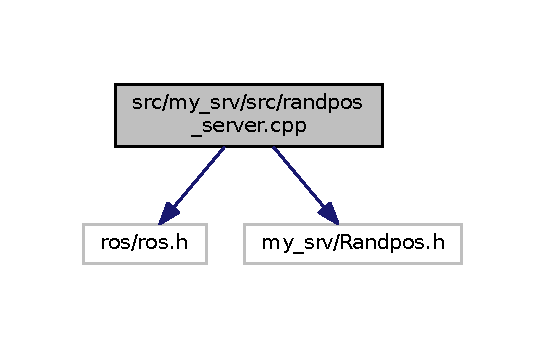
\includegraphics[width=262pt]{randpos__server_8cpp__incl}
\end{center}
\end{figure}
\subsection*{Functions}
\begin{DoxyCompactItemize}
\item 
double \hyperlink{randpos__server_8cpp_a10f83119b77a8fbd085a5550955f85ff}{rand\+M\+ToN} (double M, double N)
\item 
bool \hyperlink{randpos__server_8cpp_a76e934ac14d6efef64e827323ece1096}{position} (my\+\_\+srv\+::\+Randpos\+::\+Request \&req, my\+\_\+srv\+::\+Randpos\+::\+Response \&res)
\item 
int \hyperlink{randpos__server_8cpp_a3c04138a5bfe5d72780bb7e82a18e627}{main} (int argc, char $\ast$$\ast$argv)
\end{DoxyCompactItemize}


\subsection{Function Documentation}
\index{randpos\+\_\+server.\+cpp@{randpos\+\_\+server.\+cpp}!main@{main}}
\index{main@{main}!randpos\+\_\+server.\+cpp@{randpos\+\_\+server.\+cpp}}
\subsubsection[{\texorpdfstring{main(int argc, char $\ast$$\ast$argv)}{main(int argc, char **argv)}}]{\setlength{\rightskip}{0pt plus 5cm}int main (
\begin{DoxyParamCaption}
\item[{int}]{argc, }
\item[{char $\ast$$\ast$}]{argv}
\end{DoxyParamCaption}
)}\hypertarget{randpos__server_8cpp_a3c04138a5bfe5d72780bb7e82a18e627}{}\label{randpos__server_8cpp_a3c04138a5bfe5d72780bb7e82a18e627}
The ros\+::init() function needs to see argc and argv so that it can perform any R\+OS arguments and name remapping that were provided at the command line.

Node\+Handle is the main access point to communications with the R\+OS system.

The service is created and advertised over ros

ros\+::spin() will enter a loop \index{randpos\+\_\+server.\+cpp@{randpos\+\_\+server.\+cpp}!position@{position}}
\index{position@{position}!randpos\+\_\+server.\+cpp@{randpos\+\_\+server.\+cpp}}
\subsubsection[{\texorpdfstring{position(my\+\_\+srv\+::\+Randpos\+::\+Request \&req, my\+\_\+srv\+::\+Randpos\+::\+Response \&res)}{position(my_srv::Randpos::Request &req, my_srv::Randpos::Response &res)}}]{\setlength{\rightskip}{0pt plus 5cm}bool position (
\begin{DoxyParamCaption}
\item[{my\+\_\+srv\+::\+Randpos\+::\+Request \&}]{req, }
\item[{my\+\_\+srv\+::\+Randpos\+::\+Response \&}]{res}
\end{DoxyParamCaption}
)}\hypertarget{randpos__server_8cpp_a76e934ac14d6efef64e827323ece1096}{}\label{randpos__server_8cpp_a76e934ac14d6efef64e827323ece1096}
This function provides de service for generating random coordenates by calling the function rand\+M\+ToN to get random coordenates in x and y. It also prints them in the screen \index{randpos\+\_\+server.\+cpp@{randpos\+\_\+server.\+cpp}!rand\+M\+ToN@{rand\+M\+ToN}}
\index{rand\+M\+ToN@{rand\+M\+ToN}!randpos\+\_\+server.\+cpp@{randpos\+\_\+server.\+cpp}}
\subsubsection[{\texorpdfstring{rand\+M\+To\+N(double M, double N)}{randMToN(double M, double N)}}]{\setlength{\rightskip}{0pt plus 5cm}double rand\+M\+ToN (
\begin{DoxyParamCaption}
\item[{double}]{M, }
\item[{double}]{N}
\end{DoxyParamCaption}
)}\hypertarget{randpos__server_8cpp_a10f83119b77a8fbd085a5550955f85ff}{}\label{randpos__server_8cpp_a10f83119b77a8fbd085a5550955f85ff}
This program is conceived to work as a service server that gives back random coordinates between the specified range This function just creates and returns a random number between the minimum and maximum boundaries specified 
\hypertarget{velocity__server_8cpp}{}\section{src/my\+\_\+srv/src/velocity\+\_\+server.cpp File Reference}
\label{velocity__server_8cpp}\index{src/my\+\_\+srv/src/velocity\+\_\+server.\+cpp@{src/my\+\_\+srv/src/velocity\+\_\+server.\+cpp}}
{\ttfamily \#include \char`\"{}ros/ros.\+h\char`\"{}}\\*
{\ttfamily \#include \char`\"{}my\+\_\+srv/\+Velocity.\+h\char`\"{}}\\*
Include dependency graph for velocity\+\_\+server.\+cpp\+:
\nopagebreak
\begin{figure}[H]
\begin{center}
\leavevmode
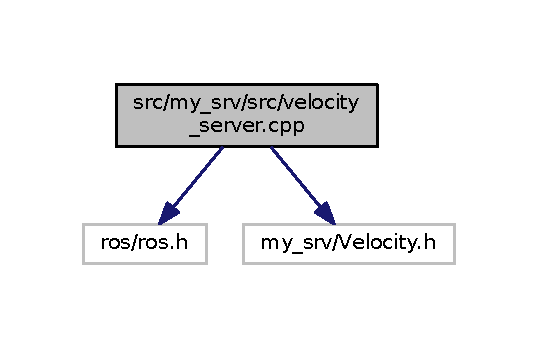
\includegraphics[width=258pt]{velocity__server_8cpp__incl}
\end{center}
\end{figure}
\subsection*{Functions}
\begin{DoxyCompactItemize}
\item 
double \hyperlink{velocity__server_8cpp_a10f83119b77a8fbd085a5550955f85ff}{rand\+M\+ToN} (double M, double N)
\item 
bool \hyperlink{velocity__server_8cpp_a976db24262bacc87ba8b6897c661c719}{myrandom} (my\+\_\+srv\+::\+Velocity\+::\+Request \&req, my\+\_\+srv\+::\+Velocity\+::\+Response \&res)
\item 
int \hyperlink{velocity__server_8cpp_a3c04138a5bfe5d72780bb7e82a18e627}{main} (int argc, char $\ast$$\ast$argv)
\end{DoxyCompactItemize}


\subsection{Function Documentation}
\index{velocity\+\_\+server.\+cpp@{velocity\+\_\+server.\+cpp}!main@{main}}
\index{main@{main}!velocity\+\_\+server.\+cpp@{velocity\+\_\+server.\+cpp}}
\subsubsection[{\texorpdfstring{main(int argc, char $\ast$$\ast$argv)}{main(int argc, char **argv)}}]{\setlength{\rightskip}{0pt plus 5cm}int main (
\begin{DoxyParamCaption}
\item[{int}]{argc, }
\item[{char $\ast$$\ast$}]{argv}
\end{DoxyParamCaption}
)}\hypertarget{velocity__server_8cpp_a3c04138a5bfe5d72780bb7e82a18e627}{}\label{velocity__server_8cpp_a3c04138a5bfe5d72780bb7e82a18e627}
\index{velocity\+\_\+server.\+cpp@{velocity\+\_\+server.\+cpp}!myrandom@{myrandom}}
\index{myrandom@{myrandom}!velocity\+\_\+server.\+cpp@{velocity\+\_\+server.\+cpp}}
\subsubsection[{\texorpdfstring{myrandom(my\+\_\+srv\+::\+Velocity\+::\+Request \&req, my\+\_\+srv\+::\+Velocity\+::\+Response \&res)}{myrandom(my_srv::Velocity::Request &req, my_srv::Velocity::Response &res)}}]{\setlength{\rightskip}{0pt plus 5cm}bool myrandom (
\begin{DoxyParamCaption}
\item[{my\+\_\+srv\+::\+Velocity\+::\+Request \&}]{req, }
\item[{my\+\_\+srv\+::\+Velocity\+::\+Response \&}]{res}
\end{DoxyParamCaption}
)}\hypertarget{velocity__server_8cpp_a976db24262bacc87ba8b6897c661c719}{}\label{velocity__server_8cpp_a976db24262bacc87ba8b6897c661c719}
\index{velocity\+\_\+server.\+cpp@{velocity\+\_\+server.\+cpp}!rand\+M\+ToN@{rand\+M\+ToN}}
\index{rand\+M\+ToN@{rand\+M\+ToN}!velocity\+\_\+server.\+cpp@{velocity\+\_\+server.\+cpp}}
\subsubsection[{\texorpdfstring{rand\+M\+To\+N(double M, double N)}{randMToN(double M, double N)}}]{\setlength{\rightskip}{0pt plus 5cm}double rand\+M\+ToN (
\begin{DoxyParamCaption}
\item[{double}]{M, }
\item[{double}]{N}
\end{DoxyParamCaption}
)}\hypertarget{velocity__server_8cpp_a10f83119b77a8fbd085a5550955f85ff}{}\label{velocity__server_8cpp_a10f83119b77a8fbd085a5550955f85ff}

%--- End generated contents ---

% Index
\backmatter
\newpage
\phantomsection
\clearemptydoublepage
\addcontentsline{toc}{chapter}{Index}
\printindex

\end{document}
